\chapter{Požadavky, analýza a návrh}
\label{chap:3}
\section{Požadavky}
\label{sec:3.1}
\subsection{Funkční požadavky}
\subsubsection{Diagram případů užití}
\begin{figure}[h!]
	\centering
	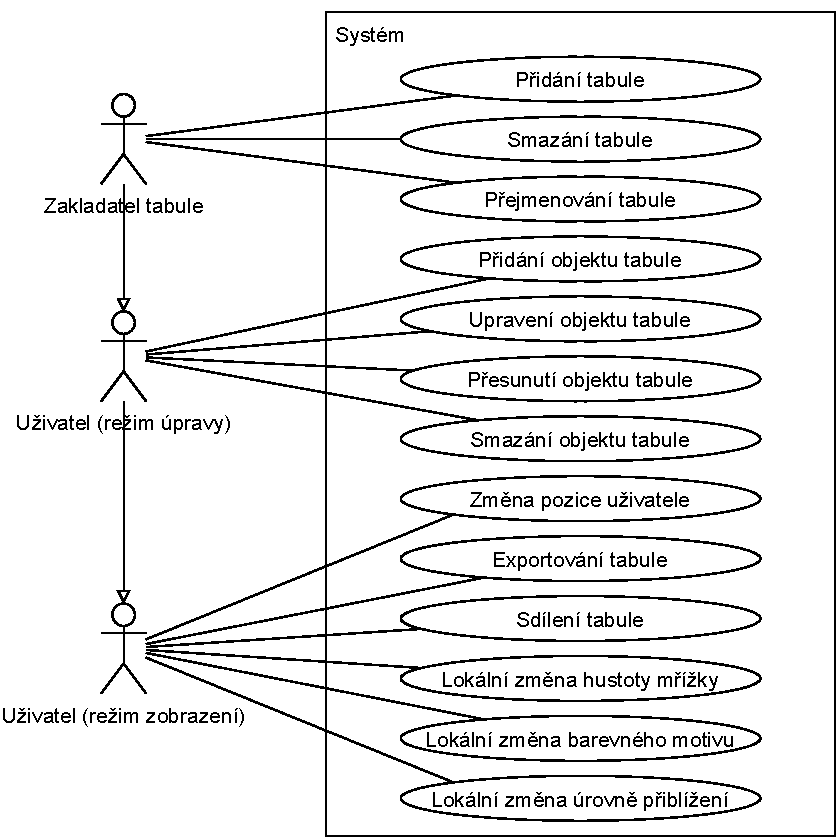
\includegraphics[width=0.6\textwidth]{Figures/UseCaseDiagram.pdf}
	\caption{Diagram případů užití}
	\label{fig:UseCaseDiagram}
\end{figure}
%#TODO Use-case / aktivitní diagram:
% + přidání tabule
% - přidání objektu tabule (lze dobře přidat rozšíření, kde bude odebrání objektu před kontrolou ID)
% - export tabule (obrázek)
% Sekvenční diagram:
% - přihlášení / připojení na tabuli
% + přidání obrázku
% - přidání zdrojového souboru
\clearpage


%#TODO\subsubsection{Scénáře případů užití}
%...


%#TODO\subsubsection{Aktivitní diagramy}
%#TODO\subsubsubsection{Aktivitní diagram - přidání tabule}
\subsection{Aktivitní diagram - přidání tabule}
\begin{figure}[h!]
	\centering
	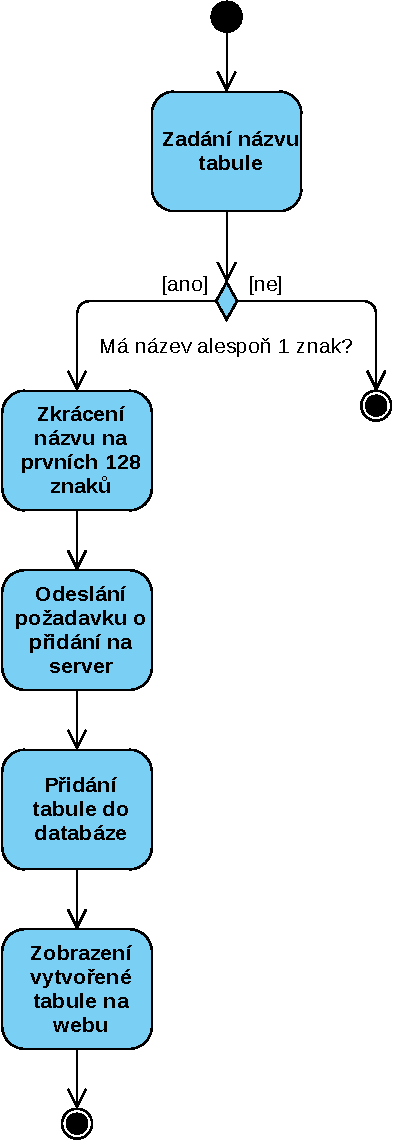
\includegraphics[width=0.33\textwidth]{Figures/ActivityDiagram1.pdf}
	\caption{Aktivitní diagram - přidání tabule}
	\label{fig:ActivityDiagram1}
\end{figure}
%#TODO...



%#TODO\subsection{Technické požadavky}
%\subsubsection{Konceptuální model domény (třídní diagram)}
%...


%#TODO\subsubsection{Odhad velikostí entit a jejich množství}
%#TODO...


%#TODO\subsubsection{Odhad počtu současně pracujících uživatelů}
%#TODO...


%#TODO\subsubsection{Typy interakcí uživatelů a odhad jejich náročnosti}
%#TODO...


%#TODO\subsubsection{Zvolené technologie a postupy}
%#TODO...
\clearpage




\section{Analýza}
\label{sec:3.2}
\subsection{Datová analýza}
\subsubsection{Relační datový model databáze}
\begin{figure}[h!]
	\centering
	%#TODO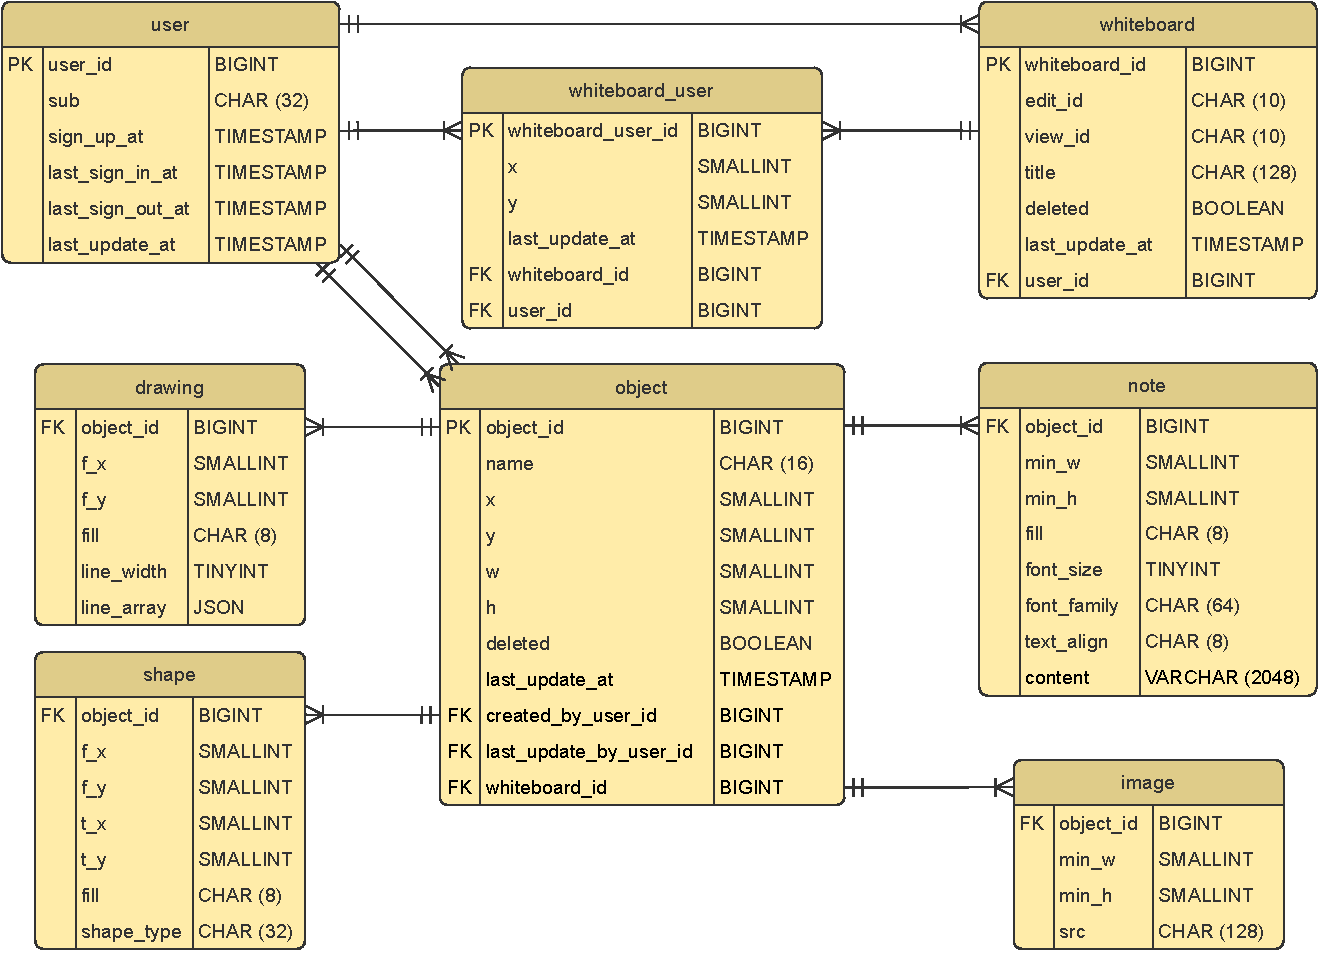
\includegraphics[width=1\textwidth]{Figures/EntityRelationshipDiagram.pdf}
	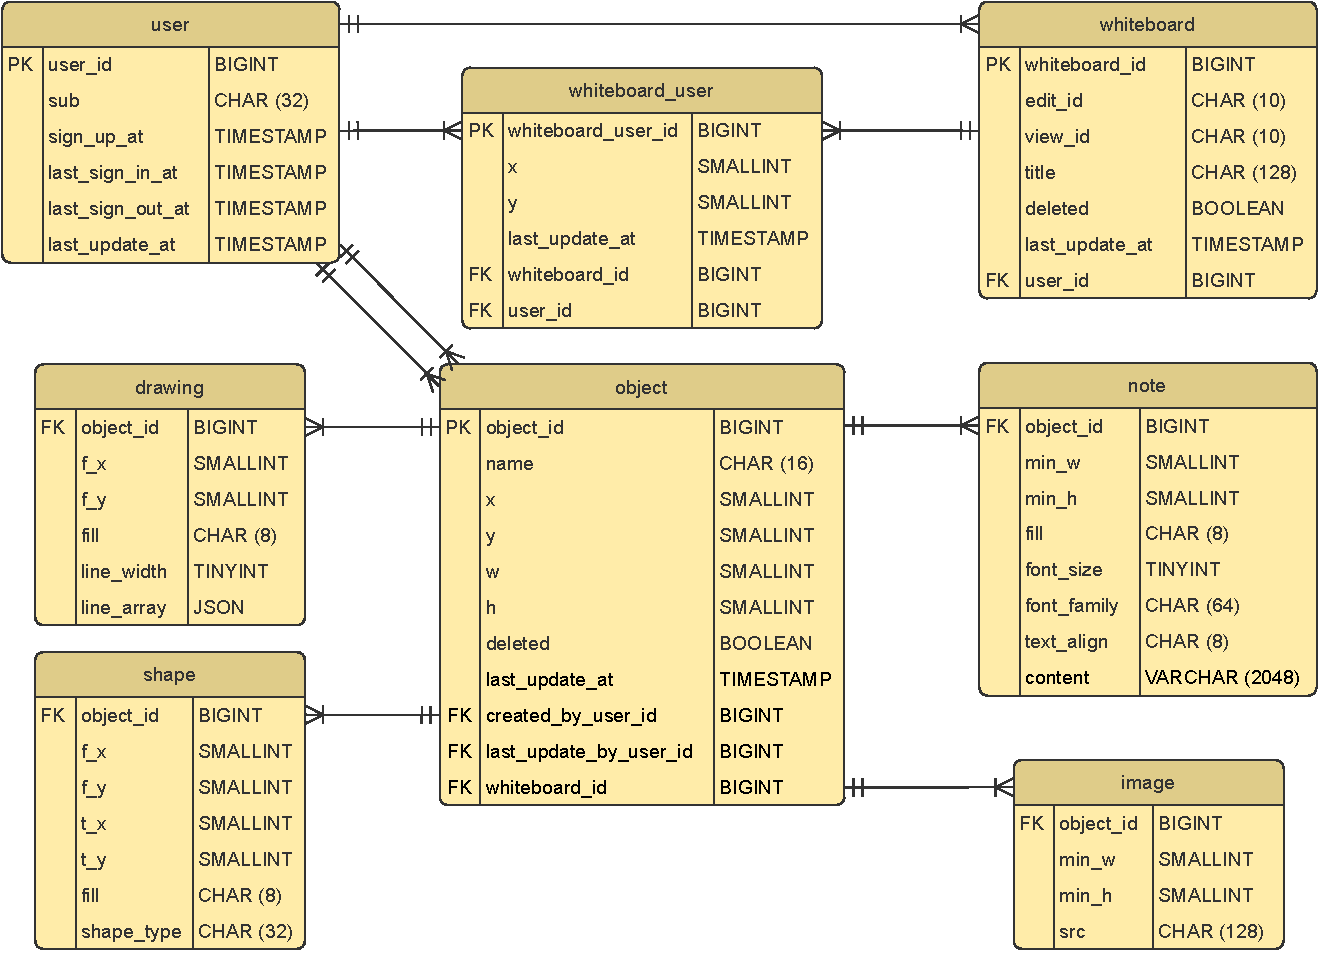
\includegraphics[width=0.9\textwidth]{Figures/EntityRelationshipDiagram.pdf}
	\caption{Relační datový model databáze}
	\label{fig:EntityRelationshipDiagram}
\end{figure}


%#TODO\subsubsection{Lineární zápis typů entit}
%#TODO...


%#TODO\subsubsection{Lineární zápis typů vztahů}
%#TODO...


%#TODO\subsubsection{Datový slovník}
%#TODO...


%#TODO\subsubsection{Integritní omezení}
%#TODO...



\subsection{Stavová analýza}
Definujeme tyto stavy tabule:
\begin{itemize}
	\item \textbf{Smazaná} -- tabule, která byla uživatelem smazána
	\item \textbf{Nesmazaná} -- tabule, která dosud nebyla uživatelem smazána
\end{itemize}

\noindent Definujeme tyto stavy objektu tabule:
\begin{itemize}
	\item \textbf{Smazaný} -- objekt tabule, který byl uživatelem smazán
	\item \textbf{Nesmazaný} -- objekt tabule, který dosud nebyl uživatelem smazán
\end{itemize}



%\subsection{Funkční analýza}
%...
\clearpage




\section{Návrh}
\label{sec:3.3}
\subsection{Architektura systému}
\subsubsection{Diagram nasazení}
\begin{figure}[h!]
	\centering
	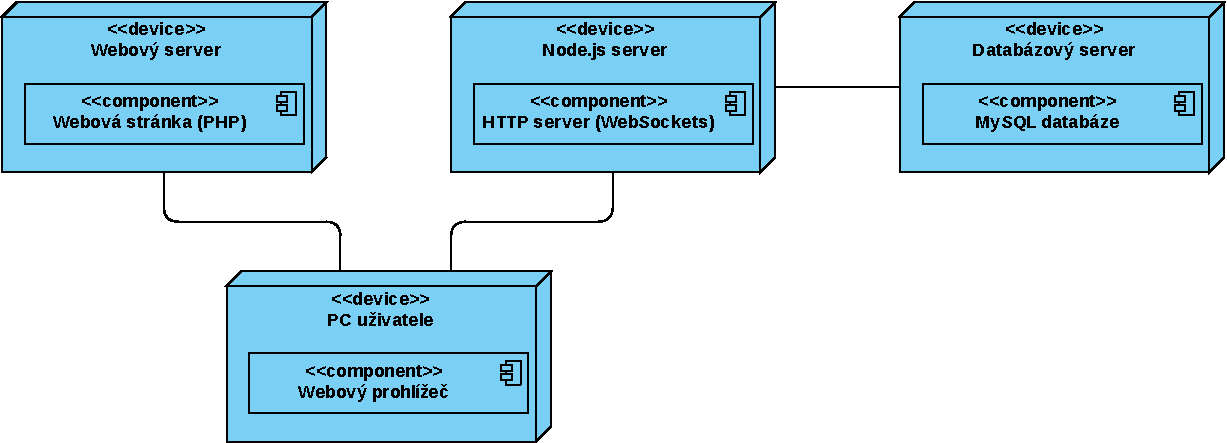
\includegraphics[width=1\textwidth]{Figures/DeploymentDiagram.pdf}
	\caption{Diagram nasazení systému}
	\label{fig:DeploymentDiagram}
\end{figure}


\subsubsection{Diagram komponent - datová komunikace}
\begin{figure}[h!]
	\centering
	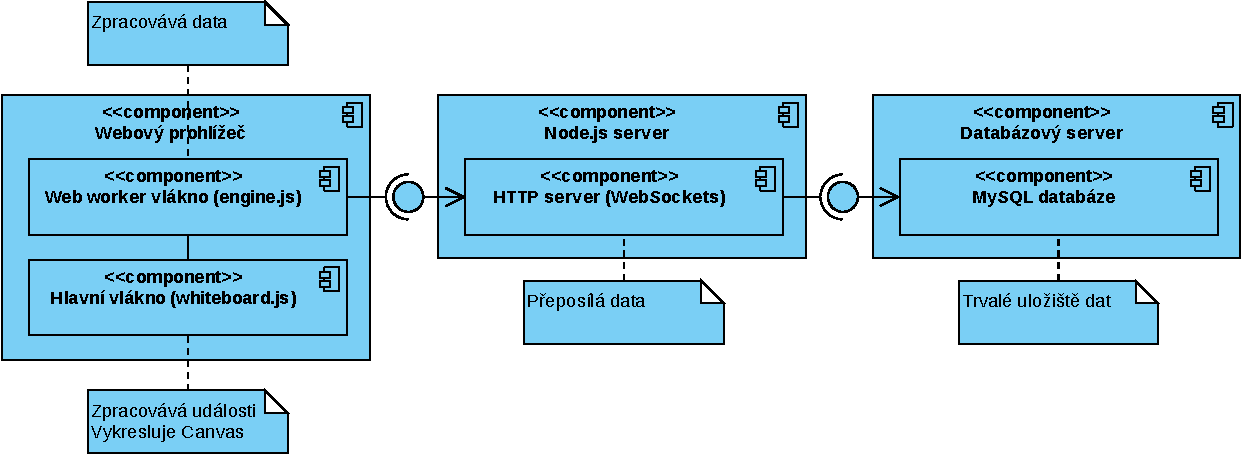
\includegraphics[width=1\textwidth]{Figures/ComponentDiagram.pdf}
	\caption{Diagram komponent - datová komunikace}
	\label{fig:ComponentDiagram}
\end{figure}
\clearpage



%#TODO\subsection{Sekvenční diagramy}
%#TODO\subsubsection{Sekvenční diagram - změna obrázku objektu tabule}
\subsection{Sekvenční diagram - změna obrázku objektu tabule}
\begin{figure}[h!]
	\centering
	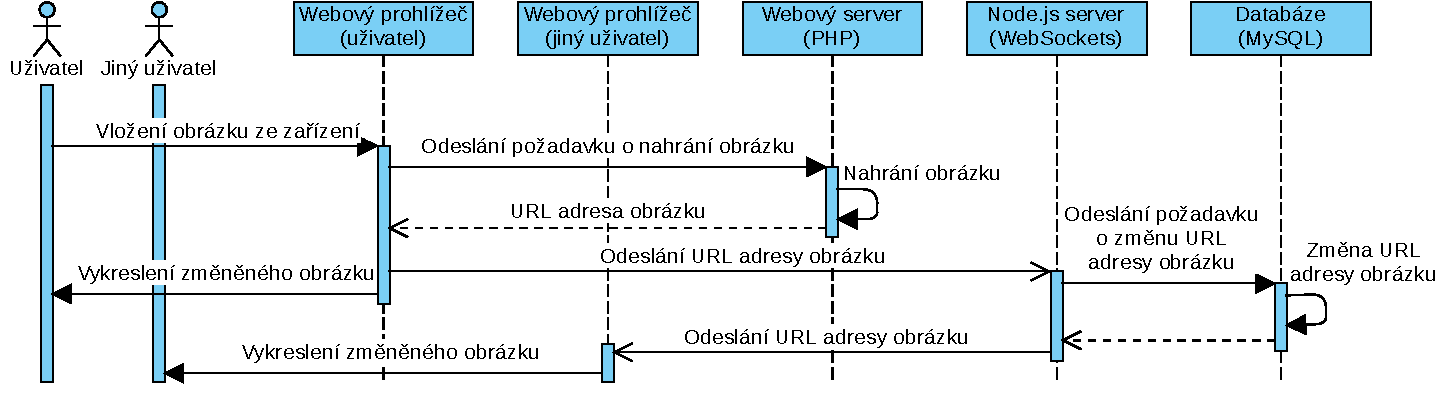
\includegraphics[width=1\textwidth]{Figures/SequenceDiagram1.pdf}
	\caption{Sekvenční diagram - změna obrázku objektu tabule}
	\label{fig:SequenceDiagram1}
\end{figure}
%#TODO...
\endinput